\documentclass{beamer}

\usepackage{graphicx}
\usepackage{pgfpages}
\usepackage{hyperref}
\usepackage[
backend=biber,
style=alphabetic,
citestyle=authoryear
]{biblatex}

\addbibresource{library.bib}

% \setbeameroption{show only notes}
\usetheme{material}

% \usePrimary{00897B}{00695C}{FFFFFF}
\usePrimaryTeal
% \useAccent{009688}{000000}
\useAccent{004D40}{000000}

\title{Core techniques of \\ \textbf{QA Systems over KBs \\ a Survey}}
\author{Guillermo Echegoyen Blanco}
\date{}

\begin{document}

\maketitle

% ToDo := TOC
% ToDO := Add SOTA for each Part
% ToDo := In the graph, DAG perspective, add images and mention Zou's graph matching
% ToDo := In Entity Linking add S-MART ?

\begin{frame}{Overview}
  \begin{card}
    \tableofcontents
  \end{card}
\end{frame}


\begin{comment}
\begin{frame}{Tasks}
  \centering
  \begin{columns}
    \setbeamercolor{coloredboxstuff}{fg=white,bg=white!10!box1}
    \begin{beamercolorbox}[wd=0.33\textwidth,sep=1em]{coloredboxstuff}
      \centering
      Question Analysis
    \end{beamercolorbox}
    \setbeamercolor{coloredboxstuff}{fg=white,bg=white!10!box2}
    \begin{beamercolorbox}[wd=0.33\textwidth,sep=1em]{coloredboxstuff}
      \centering
      Phrase Mapping
    \end{beamercolorbox}
    \setbeamercolor{coloredboxstuff}{fg=white,bg=white!10!box3}
    \begin{beamercolorbox}[wd=0.33\textwidth,sep=1em]{coloredboxstuff}
      \centering
      Disambiguation
    \end{beamercolorbox}
  \end{columns}
  \begin{columns}
    \setbeamercolor{coloredboxstuff}{fg=white,bg=white!10!box4}
    \begin{beamercolorbox}[wd=0.5\textwidth,sep=1em]{coloredboxstuff}
      \centering
      Query Construction
    \end{beamercolorbox}
    \setbeamercolor{coloredboxstuff}{fg=white,bg=white!10!box5}
    \begin{beamercolorbox}[wd=0.5\textwidth,sep=1em]{coloredboxstuff}
      \centering
      Distributed Knowledge
    \end{beamercolorbox}
  \end{columns}
\end{frame}
\end{comment}

\section{Intro}

\begin{frame}{Intro}
  \begin{cardTiny}
    \begin{itemize}
      \item A Question Answering System should be able to: \\
      \textit{Understand a Natural Language Question so as to be able to answer based on some pre-known data.}
    \end{itemize}
  \end{cardTiny}
  \begin{cardTiny}
    \begin{itemize}
      \item Typically involves accepting a question and generating a SparQL query capable of extracting the information which answers the user question.
    \end{itemize}
  \end{cardTiny}
  \begin{cardTiny}
    \begin{itemize}
      \item QALD benchmark
      \item WebQuestions benchmark
      \item SimpleQuestions benchmark
    \end{itemize}
  \end{cardTiny}
\end{frame}

\section{Tasks}

\begin{frame}{Tasks}
  \begin{card}
    \begin{itemize}
      \item Question Analysis
      \item Phrase Mapping
      \item Disambiguation
      \item Query Construction
    \end{itemize}
  \end{card}
\end{frame}

\section{Question Analysis}

% ToDo := Describe the problems here
\begin{frame}{Question Analysis \#1}
  \begin{card}
    Analyze syntactic features to extract meaningful information:
    \begin{itemize}
      \item Type of question (is it a Which, What\dots question).
      \item Multilinguality (is it in English, French\dots).
      \item Correspondance to KB entities/classes.
      \item Tokens in the sentence and it's relations.
      \item Useless words in the sentence.
    \end{itemize}
  \end{card}
\end{frame}

\begin{frame}{Question Analysis \#2}
  \begin{card}
    Techniques based on:
    \begin{itemize}
      \item Recognizing Named Entities
      \item Segmenting with $POS^{*}$ Tags
      \item Identifying dependencies using parsers
    \end{itemize}
  \end{card}
  \vspace{8em}
  POS Tag: Part-Of-Speech Tag
\end{frame}

\note[itemize]{
  % ToDo := Correct this notes
  \item Recognizing Named Entities consists in finding the entities corresponding to parts of the phrase (eg: Europe dbr:European\_Union):Which token correspond to which resource in the KB
  \item Segmenting is like tokenization of different parts of the string, where the tag is usually universal
  \item Dependencies refer to parts of the phrase which depend upon others, direct cumpliment, adjective, subjective noun\dots
}

\begin{frame}{Question Analysis \#3 - Recognizing named entities}
  \begin{card}
    Identify Named Entities and map to resource in KB
    \begin{itemize}
      \item \textit{NER} Tools: Tools from NLP, \textbf{\textit{Standford NER Tool}}. Domain specific, \textbf{low precision 51\%} (\cite{he2014a})
      \item \textit{N-Gram}: Map n-grams to KB entities. Adv: Each NE can be recognized in the KB, disadv: Dissambiguation explodes (\textbf{too much candidates}). (SINA: \cite{shekarpour2015a}, CASIA: \cite{he2014a})
      \item \textit{Entity Linking} Tools: \textbf{DBpedia Spotlight} (\cite{daiber2013a}), \textbf{DBpedia Lookup} and \textbf{AIDA} (\cite{yosef2011a}). Recognize NE and find the underlying KB resource, dissambiguating on the way. Adv: All-in-one. Disadv: Limited service, \textbf{KB dependant}.
    \end{itemize}
  \end{card}
\end{frame}

\note{
  Identify tokens in the sentence that refer to a resource in the KB, discarding useless words.
  \begin{itemize}
    \item When grouping n-grams, if an entity is found, the n-gram is considered, else more n-grams are tried.
  \end{itemize}
  Propose n-grams with attention mechanism?
}

\begin{frame}{Question Analysis \#4 - Segmenting using POS Tagging}
  \begin{card}
    Identify which phrase correspond to instances, properties, classes\dots and which is irrelevant.
    \begin{itemize}
      \item \textit{Handmade rules}: Regular expressions depenending on question type, structure\dots. (PowerAqua \cite{lopez2012a}, Treo \cite{freitas2014a}, DEANNA \cite{yahya2013a}). Disadv: \textbf{regex built by hand}.
    \end{itemize}
    \begin{figure}\label{fig:pos_tagging}
      \centering
      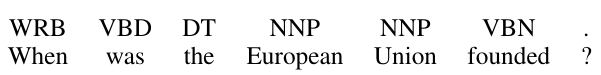
\includegraphics[width=0.8\textwidth]{./res/pos.png}
      \caption{POS tagging from the \textbf{Standford POS Tagger}}
    \end{figure}
  \end{card}
\end{frame}

\begin{frame}{question Analysis \#5 - Segmenting using POS Tagging}
  \begin{card}
    \begin{itemize}
      \item \textit{Learning rules}: \textbf{Machine Learning} approach, train over corpus (Xser \cite{xu2014a}, UTQA \cite{pouran2016a}). Disadv: \textbf{training corpus needed}.
    \end{itemize}
    \begin{figure}\label{fig:conll_tagging}
      \centering
      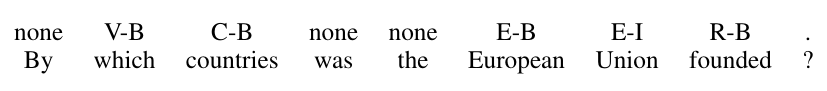
\includegraphics[width=0.9\textwidth]{./res/conll.png}
      \caption{Question annonated with \textbf{CoNLL IOB format}}
    \end{figure}
  \end{card}
\end{frame}

\note{
  It is not clear how to identify the relation between different chunks of a question
}

\begin{frame}{Question Analysis \#6 - Parsers}
  \begin{card}
    Grammar based parsers to generate trees or DAGs
    \begin{itemize}
      \item \textit{Dependency grammars}: \textbf{Standford dependency parser}, word dependencies. Adv: can extract relations along with it's arguments (gAnswer \cite{zou2014a}, \textbf{PATTY} \cite{nakashole2012a})
      \item \textit{Dependencies and DAGs}: Dependencies between phrases. Disadv: \textbf{parser trained on dataset} (Xser \cite{xu2014a}).
    \end{itemize}
  \end{card}
\end{frame}

\note{
  DAG based parser operates on a phrase level, dependency grammars on a word level.
}

\begin{frame}{Question Analysis \#7 - Summary}
  \begin{card}[Which techniques to choose?]
    \begin{itemize}
      \item Xser (\textbf{trained DAG}) reports best results on \textit{QALD 4.1 \& 5}
      \item gAnswer (\textbf{Dependency grammars}) reports fastest results on \textit{QALD 3 \& 4}
    \end{itemize}

    Machine Learning approach: Can be fast enough and there is plenty of data available.
  \end{card}
\end{frame}

\section{Phrase Mapping}

% ToDo := Add the problems here
\begin{frame}{Phrase Mapping \#1}
  \begin{card}
    Find the resources in the KB with the highest probability that maps to the phrase.
  \end{card}
  \begin{card}
    Problems:
    \begin{itemize}
      \item String similarity
      \item Semantic similarity
      \item Language
    \end{itemize}
  \end{card}
\end{frame}

\note{
  String similarity: very similar words, different meaning (which, witch)
  Semantic similarity: words with related semantic meaning but different writing (king, queen)
}

\begin{frame}{Phrase Mapping \#2}
  \begin{card}
    \begin{itemize}
      \item Database with lexicalization: \textit{WordNet, Wiktionary, PATTY} Expand the phrase with synonims and use that for search. Adv: High number of candidates, disadv: \textbf{Big search space}, \textbf{not very useful for domain specific mappings}.
      \item Mappings using large texts: \textbf{word2vec} semantics reflected in the associated vector. Adv: aids in \textbf{lexical gap, string similarity and semantic similarity}, disadv: \textbf{needs training on large texts, noisy, performance}.
    \end{itemize}
  \end{card}
\end{frame}

\note{
  PATTY is a database with relational lexicalization, uses pattern synsets (is album, [[num]] album by)
}

% ToDo := Speak about zou, phrase mapping with Subgraph matching, solves partially the Disambiguation
\begin{frame}{Phrase Mapping \#3 - Summary}
  \begin{card}[Which techniques to choose?]
    ToDo
  \end{card}
\end{frame}

\section{Dissambiguation}

\begin{frame}{Disambiguation \#1}
  \begin{card}
    QA systems generate lots of possible interpretations due to language ambiguities and search process.
    \begin{itemize}
      \item Find univocally the resource that maps to the requested question.
    \end{itemize}
  \end{card}
  \begin{card}
    Typically approached:
    \begin{itemize}
      \item String or semantic similarity to resource label (include).
      \item Consistency check between the properties and their arguments (exclude).
    \end{itemize}
  \end{card}
\end{frame}

\note{
  Local dissambiguation excluded, all systems do it. Example "Who is the director of The Lord Of the Rings?", with no information associated with the director resource, it is not possible.
}

\begin{frame}{Disambiguation \#2 - Graph Search}
  \begin{card}
    Dissambiguation carried out in the KB search step
    \begin{itemize}
      \item Subgraph matching against the KB (\textbf{gAnswer} \cite{zou2014a} does it on phrase mapping). Represent the question as a dependency graph and find an isomorfic subgraph in KB\@. Adv: very fast. Disadv: dissambiguation carries over. (\textbf{high precision, low recall})
      \item Search both with edges and nodes (\textbf{PowerAqua} \cite{lopez2012a}). Disadv: slow.
      \item \textbf{SemSek} \cite{aggarwal2012a} and \textbf{Treo} \cite{freitas2014a} do it only with recognized instances. (\textbf{low precision, high recall})
    \end{itemize}
  \end{card}
\end{frame}

\note{
  gAnswer uses scores each possible match proportionally to the distance between labels and resources, searches both in edges and nodes.

  PowerAqua does a balance between recall and precision based on the question analysis.
}

\begin{frame}{Dissambiguation \#3 - Graph Search}
  \begin{cardTiny}
    \textbf{gAnswer} searches in the edges and vertices, \textbf{SemSek, Treo} search on instances and properties attached.
    \begin{figure}\label{fig:subgraph}
      \centering
      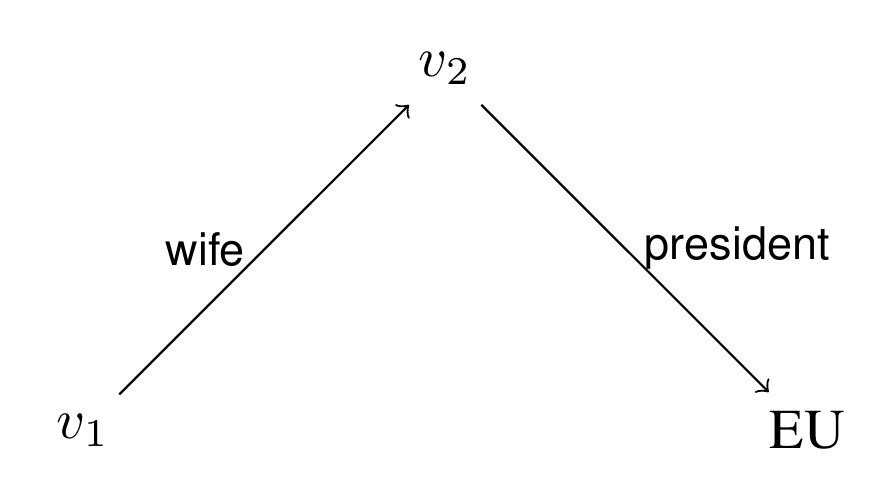
\includegraphics[height=0.45\textheight]{./res/subgraph.png}
      \caption{Subgraph generated for the question "Who is the wife of the president of the EU?"}
    \end{figure}
  \end{cardTiny}
\end{frame}

\begin{frame}{Dissambiguation \#4 - Hidden Markov Model (HMM)}
  \begin{cardTiny}
    \textit{"By which countries was the EU founded?"} \\
    Two stochastic processes:
    \begin{itemize}
      \item \textbf{Hidden (dissambiguation) $X_{t \in N}$:} \{\textit{dbo:Country, dbr:Euro, dbr:European\_Union, dbp:founded, dbp:establishedEvent}\}.
      \item \textbf{Observed (question tokens), $Y_{t \in N}$:} \{\textit{"countries", "EU", "founded"}\}.
    \end{itemize}
  \end{cardTiny}
  \begin{cardTiny}
    \begin{figure}\label{fig:hmm}
      \centering
      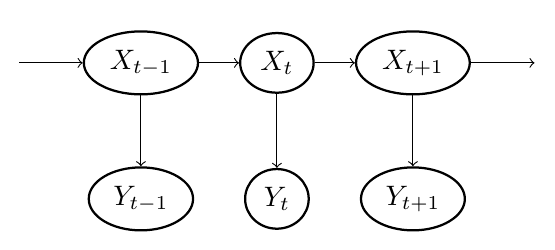
\includegraphics[height=0.30\textheight]{./res/hmm.png}
    \end{figure}
  \end{cardTiny}
\end{frame}

\note{
  This means that the appearance of a resource at time t depends only on the appearance of a resource at t -1
}

\begin{frame}{Dissambiguation \#5 - HMM}
  \begin{card}
    The problem is reduced to find the most probable set of states. Extra parameters:
    \begin{itemize}
      \item Initial probability $P(X_{0} = x)$ for $x \in X$
      \item Transition probability $P(X_{t} = x_{1} | X_{t-1} = x_{2})$ for $x_{1}, x_{2} \in X$
      \item Emission probability $P(Y_{t} = y | X_{t} = x)$ for $x \in X, y \in Y$
    \end{itemize}
    It is not necessary to know the the dependency between different resources, just the available resources.
  \end{card}
\end{frame}

\begin{frame}{Disambiguation \#6 - HMM}
  \begin{card}
    \textbf{SINA} (\cite{shekarpour2015a}): \textbf{slow}
    \begin{itemize}
      \item Emission: string similarity between label and segment.
      \item Initial \& Transition: estimated based on the distance of the resource in the KB and popularity.
    \end{itemize}
  \end{card}
  \begin{card}
    \textbf{RTV} (\cite{giannone2013a}): \textbf{inaccurate}
    \begin{itemize}
      \item Emission: word embeddings
      \item Initial \& Transition: uniform across all resources
    \end{itemize}
  \end{card}
\end{frame}

\begin{frame}{Dissambiguation \#7 - ILP \& MLN}
  \begin{card}
    ILP Optimization problem
    \begin{itemize}
      \item \textbf{DEANNA} (\cite{yahya2013a}) Dependencies between the segments have to be computed in the question analysis phase. \textbf{slow, low precision \& recall}
    \end{itemize}
  \end{card}
  \begin{card}
    Markov Logic Network
    \begin{itemize}
      \item \textbf{CASIA} (\cite{he2014a}) Hard constraints like ILP, soft constraints flexibility \textbf{training needed low precision \& recall}
    \end{itemize}
  \end{card}
\end{frame}

\begin{frame}{Dissambiguation \#8 - Structured Perceptron}
  \begin{card}
    Considering:
    \begin{itemize}
      \item Similarity of the phrase and the corresponding resource
      \item Popularity of a label for a resource
      \item Compatibility of the range and domain of a property with the arguments.
    \end{itemize}
    \textbf{Xser} (\cite{xu2014a}) Solves ambiguity \textbf{fast, training needed}
  \end{card}
\end{frame}

\begin{frame}{Dissambiguation \#9 - Summary}
  \begin{card}[Which techniques to choose]
    ToDo
  \end{card}
\end{frame}

\section{Query Construction}

\begin{frame}{Query Construction \#1 - Issues}
  \begin{cardTiny}
    Construct a \textbf{SPARQL} query that reflects user question and gets the answer. \\
    \textit{Semantic Gap}: Issues with how the information is encoded in the KB\@. One cannot deduce how the information is stored from the question.
  \end{cardTiny}
  \begin{cardTiny}
    \textit{"Which countries are in the European Union?"} \\
    Could be encoded as: \\
    \textit{dbr:Greece dbp:member dbr:European\_Union} \\
    \textit{dbr:France dbp:member dbr:European\_Union} \\
    or as: \\
    \textit{dbr:Greece dct:subj dbc:Member\_states\_of\_the\_European\_Union} \\
    \textit{dbr:France dct:subj dbc:Member\_states\_of\_the\_European\_Union} \\
    \textbf{How to search correctly}
  \end{cardTiny}
\end{frame}

\begin{frame}{Query Construction \#2}
  \begin{card}
    Approaches:
    \begin{itemize}
      \item Using templates
      \item Using information from the question analysis
      \item Using Semantic Parsers
      \item Using Machine Learning
      \item Using semantic information
    \end{itemize}
  \end{card}
\end{frame}

\begin{frame}{Query Construction \#3 - Templates}
  \begin{card}
    Templates with parts of the query to be filled, in general by triples.
    \begin{itemize}
      \item \textbf{QAKiS} (\cite{cabrio2012a}) select queries with only one triple.
      \item \textbf{ISOFT} (\cite{park2014a}) ASK over one triple, simple SELECT, COUNT and ORDER BY or FILTER.
      \item \textbf{PowerAqua} (\cite{lopez2012a}) reduces the question to one or two triples ($<=$ predicates).
    \end{itemize}
    \textbf{Very restricted questions, language is too rich, disambiguity is key}
  \end{card}
\end{frame}

\begin{frame}{Query Construction \#4 - Question Analysis}
  \begin{card}
    Most systems get the form of the query in the question analysis and phrase mapping step.
    \begin{itemize}
      \item \textbf{Freya, Intui3} (\cite{dima2014a}) resources extracted in the phrase mapping step are combined into triples.
      \item \textbf{DEANNA} (\cite{yahya2013a}) regex over POS tags in analysis step mapped to resources in phrase mapping step. ILP in dissambiguation step to get the triples.
      \item \textbf{gAnswer, QAnswer, RTV, SemGraphQA} (\cite{zou2014a}, \cite{ruseti2015a}, \cite{giannone2013a}, \cite{beaumont2015a}) extract all the possible information from the dependency graph.
    \end{itemize}
  \end{card}
\end{frame}

\note{
  \begin{itemize}
    \item gAnswer: The graph takes the form of the final query, resources associated with nodes and edges are fetched from the KB and used in the query.
    \item QAnswer: Scan dependency tree to find subgraph tokens corresponding to resouces, many graphs, local dissambiguation to get the best ones. Top ranked graph chosen for query.
    \item RTV dependency graph -> ordered list of alternated properties and non properties. Resources searched and disambiguated with HMM. 
  \end{itemize}
  Special mention to Xser (best results), next slide
}

\begin{frame}{Query Construction \#5 - Question Analysis}
  \begin{card}
    \textbf{Xser} (\cite{xu2014a}) 3 ML algorithms, two KB independant (on the question analysis phase), one KB dependant (on dissambiguation step)
    \begin{itemize}
      \item First algorithm: determines segments of the question corresponding to variables, properties, instances and classes.
      \item Second algorithm: find dependencies between phrases. (\textbf{Standford dependencies, PATTY})
      \item Third algorithm: Dissambiguation with a \textbf{Structured Perceptron} 
    \end{itemize}
  \end{card}
\end{frame}

\begin{frame}{Query Construction \#6 - Question Analysis}
  \begin{card}
    The problem with these methods is that they all \textbf{assume} that \textbf{is possible to deduce the structure of the SPARQL query from the structure of the question} without knowing how the knowledge is encoded in the KB\@.
  \end{card}
\end{frame}

\begin{frame}{Query Construction \#7 - Semantic Parsing}
  \begin{card}
    Compose a grammar and use it to extract structure from the query.
    \begin{itemize}
      \item \textbf{G}rammatical \textbf{F}ramework (\textbf{GFMed} \cite{marginean2017a})
      \item \textbf{F}eature-based \textbf{C}ontext \textbf{F}ree \textbf{G}rammar (\textbf{TR Discover}, \cite{song2015a})
      \item \textbf{C}ombinatorial \textbf{C}ategorial \textbf{G}rammar (\cite{hakimov2015a})
      \item \textbf{L}exical \textbf{T}ree \textbf{A}djoint \textbf{G}rammar (\textbf{TBSL} \cite{unger2012a}, \textbf{BELA} \cite{walter2012a})
    \end{itemize}
  \end{card}
\end{frame}

\begin{frame}{Query Construction \#8 - Semantic Parsing}
  \begin{cardTiny}
    Question has to be well formulated. For each lexical item a corresponding semantic representation is needed. (ie \texit{married} has to map with \textit{dbo:spouse}). Learning corpus (\cite{hakimov2015a}) or from POS tags (\cite{unger2012a}). In general, \textbf{low recall}
  \end{cardTiny}
  \begin{cardTiny}
    \begin{figure}\label{fig:semantic_query}
      \centering
      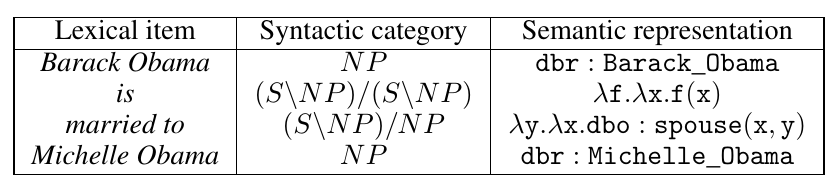
\includegraphics[width=0.85\textwidth]{./res/semantic_query.png}
      \caption{Semantic parsed question \textit{"Barack Obama is married to Michelle Obama"}}
    \end{figure}
  \end{cardTiny}
\end{frame}

\begin{frame}{Query Construction \#9 - Machine Learning}
  \begin{card}
    \textbf{CASIA} (\cite{he2014a}) (\textbf{low recall \& precision})
    \begin{itemize}
      \item Question Analysis step: extract features like position of a phrase and POS tags or the type of dependency in the dependency tree 
      \item Phrase Mapping step: associate resources with phrase segments and extract more features
      \item Dissambiguation step: MLN with extracted features to find most probable relation between segments and most probable mapping. \textbf{retrained for each KB}
    \end{itemize}
  \end{card}
\end{frame}

\begin{frame}{Query Construction \#10 - Semantic information}
  \begin{card}
    \textbf{SINA} (\cite{shekarpour2015a}), \textbf{POMELO} (\cite{hamon2014a}), \cite{zhang2016a} do not rely on the syntactic features of the question, instead the whole process is done based on the KB, just with semantic information. \\
    Advantages:
    \begin{itemize}
      \item \textbf{high recall, \& precision}
    \end{itemize}
    Disadvantages:
    \begin{itemize}
      \item \textbf{computationally expensive}
      \item \textbf{does not respect user question syntax}. No difference between \textit{"Who is the mother of Angela Merkel?"} and \textit{"Angela Merkel is the mother of who?"}
    \end{itemize}
  \end{card}
\end{frame}

\begin{frame}{Query Construction \#11 - Summary}
  \begin{card}[Which techniques to choose?]
  \end{card}
\end{frame}

\section{Conclusions}

\begin{frame}{Conclusions}
\end{frame}

\section{End}

\begin{frame}{The End}
  \begin{card}
    \centering
    \textbf{Thank you!}
  \end{card}
  \begin{card}
    \centering
    Questions?
  \end{card}
\end{frame}

\section{References}

\begin{frame}[allowframebreaks]{References}
    \printbibliography
\end{frame}

\end{document}
